\documentclass[a4paper,12pt, final]{report}
\usepackage{graphicx}
\usepackage{float}
\usepackage{url}
%\usepackage[nomain,acronym,xindy,toc]{glossaries} % nomain, if you define glossaries in a file, and you use \include{INP-00-glossary}
%\makeglossaries
%\usepackage[xindy]{imakeidx}
%\makeindex
%\usepackage[section]{placeins}
\renewcommand\bibname{References}
\usepackage[utf8]{inputenc}
%\usepackage{algorithm2e}
%\usepackage{wrapfig}
\usepackage{epsfig}
%\usepackage{hyperref}
\usepackage[hidelinks]{hyperref} % To Hide the box around links
\renewcommand\bibname{References}
%\usepackage{algorithm2e}
\usepackage{color}
\usepackage{textcomp}
\usepackage{acronym}
\usepackage[top=0.5in, bottom=1in, left=1in, right=1in]{geometry}
\usepackage{xcolor}
\definecolor{dark-red}{rgb}{0.4,0.15,0.15}
\definecolor{dark-blue}{rgb}{0.15,0.15,0.4}
\definecolor{medium-blue}{rgb}{0,0,0.5}

\newcommand{\BigO}[1]{\ensuremath{\operatorname{O}\bigl(#1\bigr)}}
\parindent 8pt
\begin{document}
  \thispagestyle{empty}
  \vspace*{1cm}
  {\centering     
  \textbf{\LARGE Exploiting ILP \& TLP using Heterogeneous-ISA Dynamic Multicore}\\
  \vspace{1.20cm}
  %\it
  %\vspace{.5cm}
  %\rm
  \textbf{\large Dual Degree Project Stage 1 Report}\\
  \vspace{1cm}
  {Submitted in partial fulfillment of the requirements}\\
  \vspace{0.25cm}
  {for the}\\
  \vspace{1cm}
  \textbf{Dual Degree Programme}\\
  \vspace{1.50cm}
  {by}\\
  \vspace{0.20cm}
  \textbf{\large Prakhar Diwan}\\
  \vspace{0.25cm}
  \textbf{\large (Roll No. 180100083)}\\
  \vspace{1.8cm}
  {Under the guidance of}\\
  \vspace{0.20cm}
  \textbf{\large Prof. Virendra Singh}\\
    \vspace{0.30cm}
  \vspace{1.450cm}
    \begin{figure}[htb]
    \begin{center}
    
\includegraphics[height=1.5in,width=1.5in]{iitblogo.png}
    \end{center}
    \end{figure}

    
  {\textbf{Department of Electrical Engineering}}\\
  {\textbf{Indian Institute of Technology Bombay}}\\
  {\textbf{October 2022}}
 
 }
 
\renewcommand{\abstractname}{Acknowledgement}
\begin{abstract}
I express my gratitude to my guide Prof. Virendra Singh for providing me the opportunity to work on this topic. I am also grateful to Nirmal Kumar Boran and other members of Computer Architecture \& Dependable Systems Lab (CADSL) for their support.  
\\\\
\\\\
\\\\
Prakhar Diwan\\
Electrical Engineering\\
IIT Bombay\\\

\end{abstract}


\clearpage 
\renewcommand{\abstractname}{Abstract} 
\abstract{
% Part on Heterogoneity in microarchitecture... 
Modern workloads demand a microarchitecture that can adapt to software diversity by exploiting instruction level parallelism (ILP) from thier sequential and thread level parallelism (TLP) from their parallel phases to achieve high performance and energy efficiency. To solve this post-multicore various reconfigurable and heterogeneous multicore architectures have been proposed which utilize heterogeneity in microarchitecture. 
% Part on ISA
Prior research has shown ISA as another dimension of heterogeneity, provides significant performance and energy efficiency gains over single-ISA heterogeneous architectures. \\     
% combining both -> this work
\indent This work proposes a reconfigurable heterogeneous-ISA dynamic multicore (HIDM) architecture aiming to exploit the heterogeneity in ISA and microarchitecture to achieve high performance and energy efficiency for both single \& multi-threaded workloads. It has promise as workload phases will get scheduled on optimal configuration (reconfigured at runtime) with respect to ISA affinity \& ILP-TLP tradeoffs. 
}

\tableofcontents
  \addcontentsline{toc}{chapter}{\listfigurename}
  \listoffigures
%  \printglossaries

%\newglossaryentry{ILP}
%{name = ILP,
%description = Instruction Level Parallelism}
\chapter{Introduction}
During the concluding decades of previous century, the major aim of microprocessor technology was to make the core faster. This was achieved through semiconductor technology advancements and architectural innovations. However, by the end of last century the power density became equal to that of the hot plate restricting further increase in frequency for performance.
\begin{figure}[H]
    \centering
    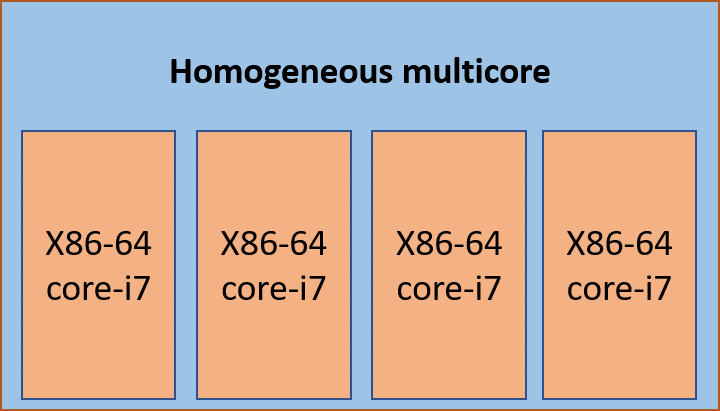
\includegraphics[width=0.5\linewidth]{homogeneous-mc.png}
    \caption{Homogeneous Multicore}
    \label{homo-mc}
\end{figure}
\indent The above limitation called "power wall" forced the designers to shift to novel architectures. To better cater the need of applications, researchers came up with multicore systems. By exploiting Thread Level Parallelism (TLP) of multi-threaded workloads through multiple cores overall performance was improved. But it saturated with single-threaded fraction of workloads becoming the bottleneck\cite{oldamdahl}. Also it leads to increase in energy consumption due to multiple cores. 
\begin{figure}[H]
    \centering
    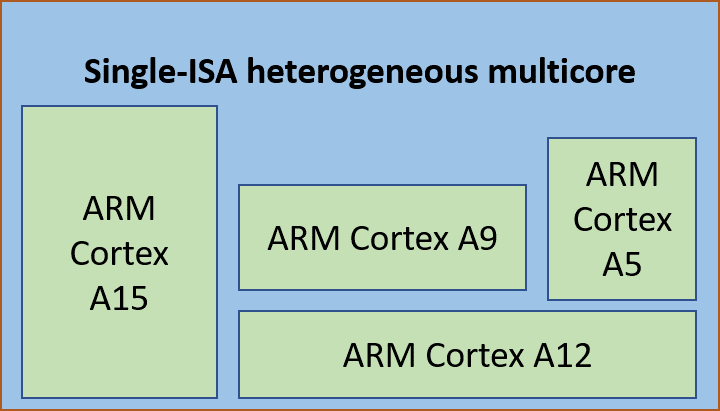
\includegraphics[width=0.5\linewidth]{single-isa-heterogeneous-mc.png}
    \caption{Single-ISA Heterogeneous Multicore}
    \label{sing-isa-hetero}
\end{figure}
\indent Initial proposed multicore architecture comprised of identical cores (Figure \ref{homo-mc}). Prior research has shown that exploiting heterogeneity is beneficial for system's performance\cite{kumarheteroperf} \& power\cite{kumarheteropower}. Architects utilised the heterogeneity in two dimensions, first was using specialized cores for certain workloads (eg: SIMD support), and second was using cores with different microarchitectures (Figure \ref{sing-isa-hetero}) based on workload's needs, to extract high performance \& energy efficiency.\\\\
\indent Till early 2010s, the heterogeneity exploration was limited to single-ISA due to high migration cost between heterogeneous-ISA systems. DeVuyst et al. \cite{DeVuystVT12} solves the problem of migration between heterogeneous-ISA cores, and Venkat et al. \cite{venkat} highlighted the benefits brought by heterogeneous-ISA multicore (Figure \ref{hetero-isa-mc}).
\begin{figure}[H]
    \centering
    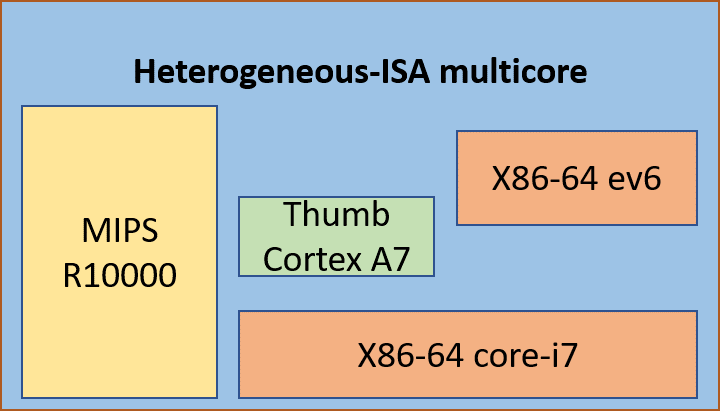
\includegraphics[width=0.5\linewidth]{hetero-isa-mc.png}
    \caption{Heterogeneous-ISA Multicore}
    \label{hetero-isa-mc}
\end{figure}
\indent Another direction of research for improvement of single-threaded performance in multicore systems was reconfigurable chip multiprocessors, where group of independent cores can dynamically morph into a large core. These architectures were capable of exploiting Instruction Level Parallelism (ILP) in sequential phases of code by using the large core, and effectively utilize TLP from parallel phases by operating as independent small cores. These type of architectures are unexplored for heterogeneous-ISA cores. \\\\
\indent Heterogeneous-ISA Dynamic Core (HIDC) has already been proposed, which exploited ISA (ARM,X86) and microarchitectural heterogeneity. The next chapter describes the research on dynamic \& heterogeneous multicore architectures. Based upon the observations from literature review, Heterogeneous-ISA Dynamic Multicore (HIDM) is proposed. It is a reconfigurable multicore architecture aimed to achieve high performance \& energy efficiency. It is expected to perform well for single-threaded (SPEC CPU2006 suite \cite{speccpu}) as well as multi-threaded workloads (PARSEC suite \cite{parsec}) by dynamically catering to ILP \& TLP needs.\\
\indent 
\chapter{Literature Review}
This chapter describes the previous work on heterogeneous multicore architectures. The first section gives insight on various ways microarchitectural heterogeneity has been exploited by summarizing some proposed ideas. The second section discusses proposals associated with ISA heterogeneity: solution to migration between heterogeneous ISA cores, harnessing performance and energy benefits from ISA diversity, and claims towards ISA homogeneity.  
\section{Heterogeneity in Microarchitecture}
\begin{figure}[H]
    \centering
    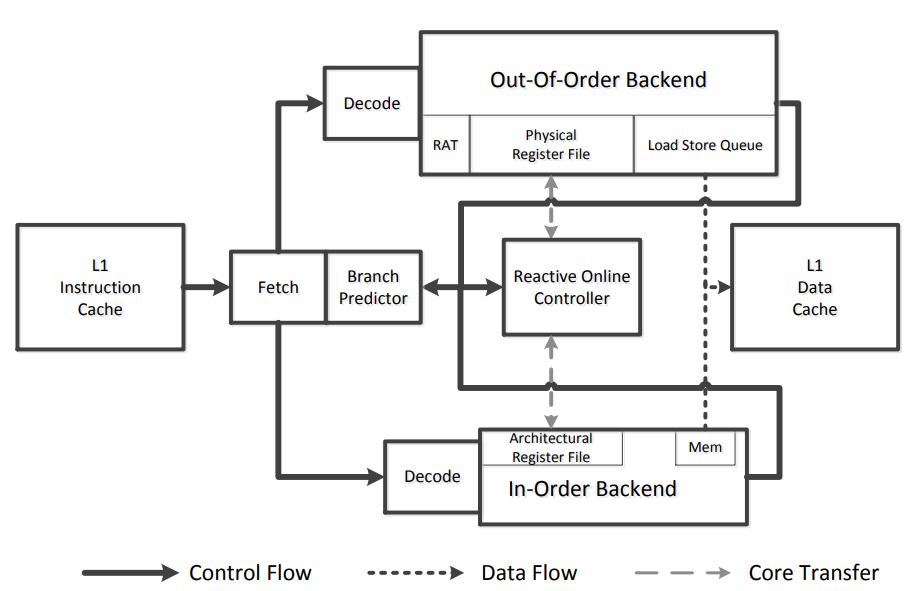
\includegraphics[width=0.65\linewidth]{composite-cores-arch.png}
    \caption{Composite Cores Architecture}
    \label{composite-arch}
\end{figure}
% Composite Cores.. 
Lukefahr et al. \cite{lukefahr2012composite} proposed Composite Cores, an architecture which reduced migration overheads by accommodating heterogeneity within a core. The core consisted of a big (out-of-order) and a little (in-order) compute $\mu$engines (Figure \ref{composite-arch}). Both shared most of the architectural state leading to reduction in data to be transferred during migration between them, which led to lower switching overheads enabling fine-grained matching of application characteristics. An online reactive controller is used for making switching decisions, aiming to maximize energy savings under user configurable performance degradation constraint. It uses linear regression model to predict CPI (cycles per instruction) for the $\mu$engine not being used in current phase, and compares the CPI difference against dynamic CPI threshold, if larger execution is done on big $\mu$engine else on little $\mu$engine. Overall 18\% energy savings were reported with performance degradation limited at 5\%. \\\\
% Morph Cores.. 
\indent Suleman et al. \cite{suleman2012morphcore} came up with the idea of MorphCore, an adaptive core microarchitecture to achieve high performance for single-threaded code and high throughput for multi-threaded code with no energy overheads. A large 2-way SMT (simultaneous multi-threading) out-of-order (OoO) core (capable of exploiting ILP) is used as the base substrate. Upon it minimal modifications are done to dynamically form a 8 SMT in-order (InO) core. Hence it provides two modes of execution (Figure \ref{morph-arch}): OoO and InO, and uses OoO mode (2-way SMT OoO core) for single-threaded code to provide high performance of a traditional OoO core with minimal degradation. For multithreaded code, it uses the InO mode (8-way SMT InO core) which provides same or better performance as an OoO core \cite{hily1999} and consumes less power. Due to no migration of instructions and data needed, switching overhead is low. Over a 2-way SMT OoO core MorphCore leads to 10\% performance improvement and 22\% reduction in energy-delay squared product. 
\begin{figure}[H]
    \centering
    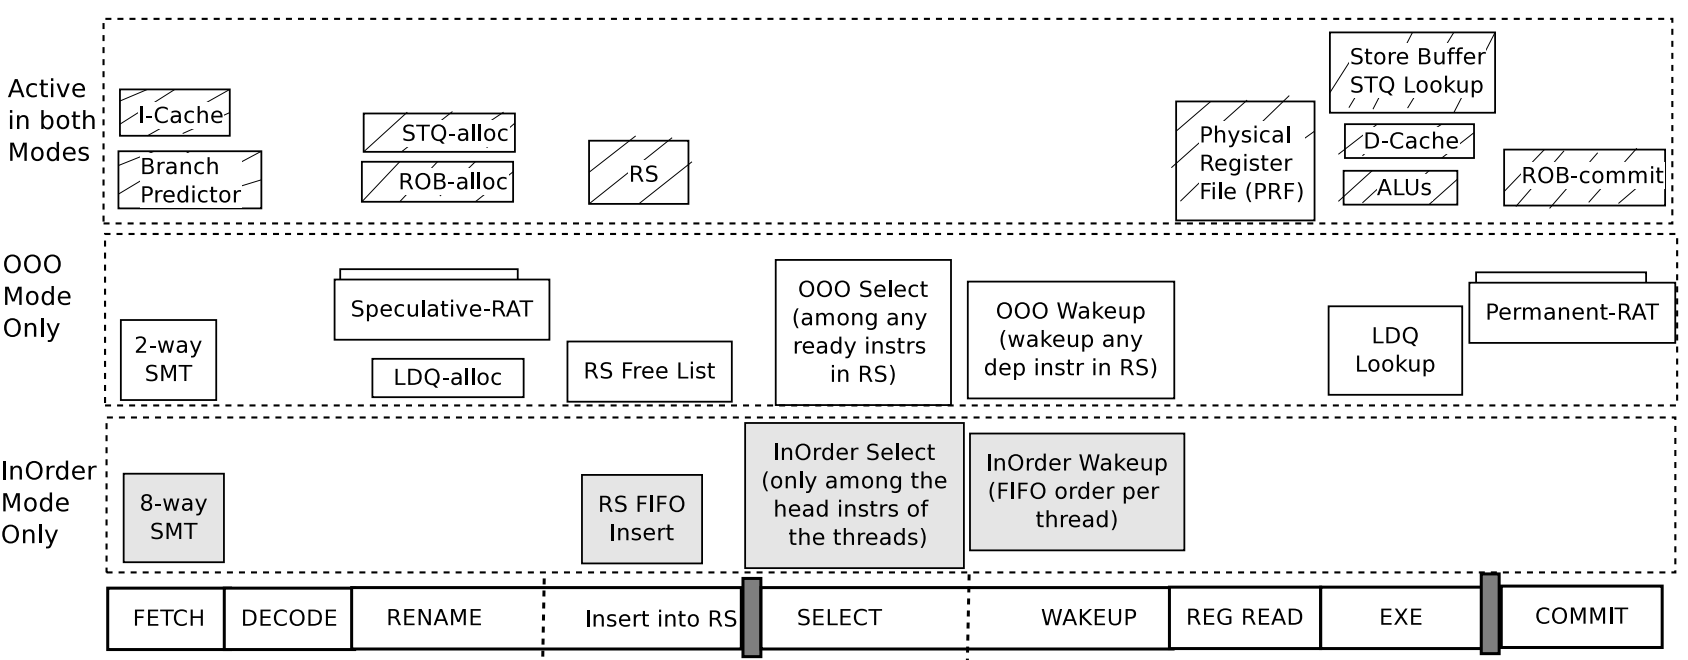
\includegraphics[width=\linewidth]{morph-uarch.png}
    \caption{MorphCore Microarchitecture}
    \label{morph-arch}
\end{figure}
% Core Fusion ..
\indent Ipek et al. \cite{ipek2007core} presented core fusion, a reconfigurable chip multiprocessor (CMP) architecture which empowers groups of fundamentally independent CMP cores with the ability to "fuse" into a large CPU on demand from application. To effectively exploit ILP from sequential phases of application, it uses the fused mode configuration to create a large core, and for parallel phases it utilizes independent mode (base multicore). It is a fully hardware-based solution which uses hints from applications itself for making reconfiguration decisions. The CMP architecture  consists of eight two-issue OoO cores
\begin{figure}[H]
    \centering
    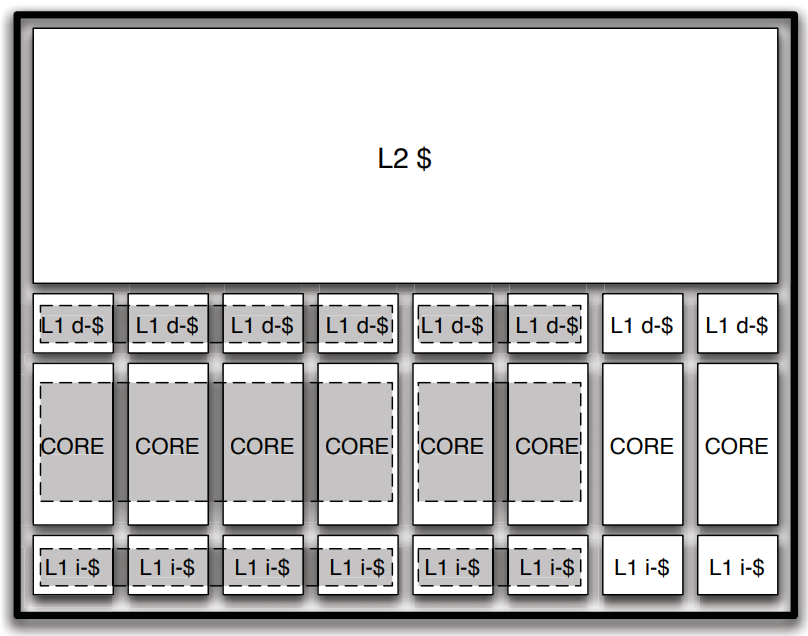
\includegraphics[width=0.5\linewidth]{corefusion-architecture.png}
    \caption{Core Fusion Conceptual Floorplan}
    \label{corefusion-arch}
\end{figure}
\noindent with private L1-i and L1-d caches and common L2 cache, the figure \ref{corefusion-arch} shows an example configuration of core fusion: one eight-issue (group of four CMP cores), one four-issue (group of two CMP cores) and two two-issue cores. Based on results shown for sequential, parallel and incrementally parallelized workloads, it was concluded that core fusion accommodates software diversity gracefully. 
\begin{figure}[H]
    \centering
    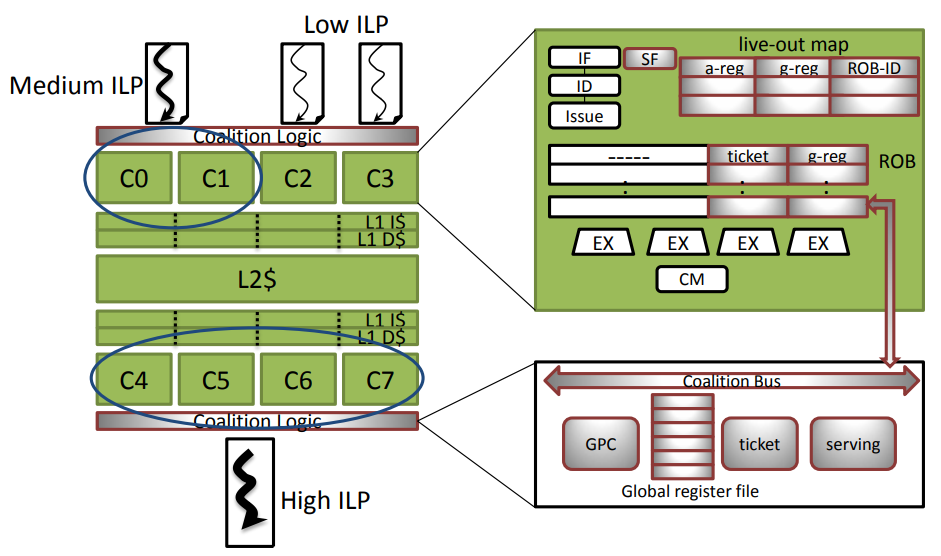
\includegraphics[width=0.7\linewidth]{bahurupi-architecture.png}
    \caption{Bahurupi Architecture}
    \label{bahurupi-arch}
\end{figure}
% Bahurupi .. 
\indent Pricopi et al. \cite{pricopi2012bahurupi} proposed another reconfigurable homogeneous multicore architecture (comprising identical 2-way OoO cores), called Bahurupi that can satisfy the conflicting demands of ILP and TLP put forth by workloads comprising fractions of parallel and serial codes. As shown in the figure \ref{bahurupi-arch}, a high ILP application is accelerated by execution on a large core dynamically composed of four CMP-cores, a medium ILP application is run on 2-core coalition and low ILP applications run on individual CMP cores. This architecture (compiler-hardware mixed solution) achieved performance of complex OoO superscalar core without paying for complex hardware and associated energy inefficiency. It's quad-core cluster reported 17\% and 43\% improvement in performance and energy consumption respectively compared to 8-way OoO core on embedded benchmark applications.
\section{Heterogeneity in ISA}
% How execution migration become possible.. 2012 DeVuyst
Devuyst et al. \cite{DeVuystVT12} claimed ISA diversity as an important dimension to gain performance using heterogeneity in cores. Multiple reasons for migration need were mentioned such as higher priority process being scheduled to high performance core with its currently executing process migrated to energy-efficient core or the process from high performance is switched to energy efficient core in battery saver mode. Authors listed various methods used during heterogeneous-ISA migration to reduce the overhead. They have modified compiler back end significantly to produce programs that keep most of their state in architectural neutral form. For maintaining stack consistency a stack transformer is used during migration. And for enabling instantaneous migration a binary translator is modified as required by the work and utilized. \\\\
\indent Venkat et al. \cite{venkat} carried out the design space exploration for finding optimal design to propose a heterogeneous-ISA CMP for general purpose computing.
Various parameters affected by ISA diversity and their impact on performance was analyzed. The program was migrated between different ISA cores at equivalence points. In case not at equivalence point, the program is binary translated to the target ISA (to be migrated to) till the nearest equivalence point is reached in execution. Authors examined phase wise affinity for various program phases and obtained execution times taken for switching between different ISA cores. Upon scheduling the program phases on the best-suited core using oracle scheduler, improvements of 20.8\% in performance and 23\% in energy efficiency were observed over single-ISA design. \\\\
% Harnessing ISA diversity work.. add some results here.. 
% Power struggles.. need to criticize the paper's result and conclude that ISA heterogeneity does matter.. 
\indent Blem et al. \cite{blempower} tried to find if the ISA plays an intrinsic role in performance and energy efficiency of the implemented system. For this authors performed detailed experiments by running real applications from various workloads on real hardware, and analysed the measurements to claim that ISA being RISC or CISC doesn't matter. However, this is not true as: using real hardware led to microarchitecural differences among considered systems, the platform utilized was not uniform across the four implementations, no ISA-specific compiler optimizations were performed for binaries, approximate scaling models have been used for frequency and technology nodes, plus these don't consider the type of transistor technology used like MOSFET, FinFET, CasFET etc. and many other reasons. Authors themselves listed multiple other infrastructural limitations in the paper. The claim made is weak as ARM and X86 systems aren't provided equal stages to be compared justly. \\\\ \indent The next chapter describes the proposed work: introducing the problem, completed work and work to be done.
\chapter{Proposed Work}
\section{Introduction}
Based upon the observations from literature review, Heterogeneous-ISA Dynamic Multicore (HIDM), a reconfigurable CMP architecture is proposed to achieve high performance \& energy efficiency, by meeting ILP-TLP \& ISA affinity needs at runtime. ARM and X86 are the 2 ISAs considered based on their current popularity. As the base core, we will use Heterogeneous ISA Dynamic Core's (8-way OoO) smaller version (2-way OoO). For analysing the performance of merged cores, we will be using corresponding multiplied width core, like group of 2 2-way OoO cores modelled using a 4-way core. This is conservative based on results from Bahurupi \cite{pricopi2012bahurupi}. \\
\indent Another proposal is to make each of the 2-way OoO core into an 8-way SMT InO core for highly threaded applications, this has been shown by Suleman et al. \cite{suleman2012morphcore}. This will help in extending the performance and energy benefits of reconfigurabilty for higher number of threads (32 for a 4 core system).  
\section{Completed Work}
Conducted an extensive literature review on various multicore architectures.
Installed the \texttt{gem5} simulator \cite{gem5} and ran simple experiments for familiarization.
Setup of full system mode simulation environment for \texttt{ARM} and \texttt{X86} configurations. \\\\
Compiled the original 13 workloads from PARSEC \cite{parsec} suite using \texttt{gcc 5.5.0} for \texttt{ARM} and \texttt{X86} ISAs. I faced issues with compilation of some benchmarks, as the suite was last updated in 2011 where they used \texttt{gcc 4.2.1} (unsupported). Also as majority of benchmarks use \texttt{pthreads} library I have chosen to use it, but it doesn't support \texttt{freqmine} benchmark. As a result some of the benchmarks will be missing in analysis from the 13 original benchmarks. \\\\ 
For choosing the optimal configuration in reconfigurable multicore architecture it is required to obtain the active number of threads at runtime, as done in work by Suleman et al. \cite{suleman2012morphcore}. Exhaustive search was performed inside documentation and web to obtain this by modifying \texttt{gem5}, but as in full system mode the kernel is provided by the user as a binary along with the disk image, it led to failure. Kernel handles the thread scheduling and has this information but wasn't able to recover it, I did backtrace the \texttt{activateContext} and \texttt{suspendContext} functions but that led to various functions, ending with stream of calls from shared libraries. I investigated the functions but it led to nowhere. But through gem5 I was able to obtain the number of physical threads (same as number of active cores) at runtime. \\\\
Then I made minimal modifications to the benchmarks to incorporate a thread counter which decremented on every thread termination thus depicting the number of live threads at runtime. The counter was a global variable set to number of threads created by the user, and was decremented in the critical section formed using mutex locks and unlocks from \texttt{pthread} library. This addition makes negligible difference in results, it was confirmed from test run of \texttt{blackscholes} benchmark with medium dataset on \texttt{ARM} simulated machine. I have tested this approach (for counting threads) for \texttt{blackscholes, bodytrack \& canneal} benchmarks. \\\\
For the X86 FS simulations I used an available disk image with the compiled binaries from PARSEC 2.1 suite earlier for testing purpose. But now as I need to perform edits in the benchmarks, I'll have to compile them. I tried doing this using host machine (X86), but the application when run on simulated machine gave \texttt{glibc} version issue.
\section{Work to be done}
\begin{itemize}
    \item Experiments on ILP-TLP trade-offs: Running PARSEC benchmarks: with 4 threads on system with 4 2-way OoO cores; with 2 threads on system with 2 4-way OoO cores; with 1 thread (or serial) on system with 1 8-way OoO core. 
    \item Appropriate compilation of PARSEC 3.0 benchmarks for X86 ISA so that it works for gem5 simulated machine. (host machine compiled application gave \texttt{glibc} version issue on simulated machine)
    \item Obtaining dynamic instruction count after every \texttt{mutex\_unlock} and dumping the simulation statistics. For this need to check the address of this function from disassembly of compiled binary, and check whenever this address is accessed and get the dynamic instruction count.
    \item Scripting files for running PARSEC benchmarks with varying number of threads and the underlying system configurations 
    \item Analysis of statistics for each phase run on each configuration to determine optima. Approximation of reconfiguration delays
\end{itemize}
%\section{Simulation Results}
%\chapter{Conclusion \& Future scope}
\bibliographystyle{ieeetr}
\bibliography{thesisTemplate}{}
\end{document}
